\chapter{Introducción}

\section{Contexto}

El avance tecnológico ha impulsado la integración de arquitecturas distribuidas, inteligencia artificial y procesamiento de lenguaje natural en soluciones educativas y empresariales. En este contexto, los sistemas basados en arquitectura cliente-servidor permiten una separación eficiente entre las capas de presentación y lógica de negocio, facilitando la escalabilidad, el mantenimiento y la integración de servicios externos como OpenAI y Google Text-to-Speech. Todo debe estar citado correctamente \cite{doe2023}.

\begin{figure}[ht]
  \centering
  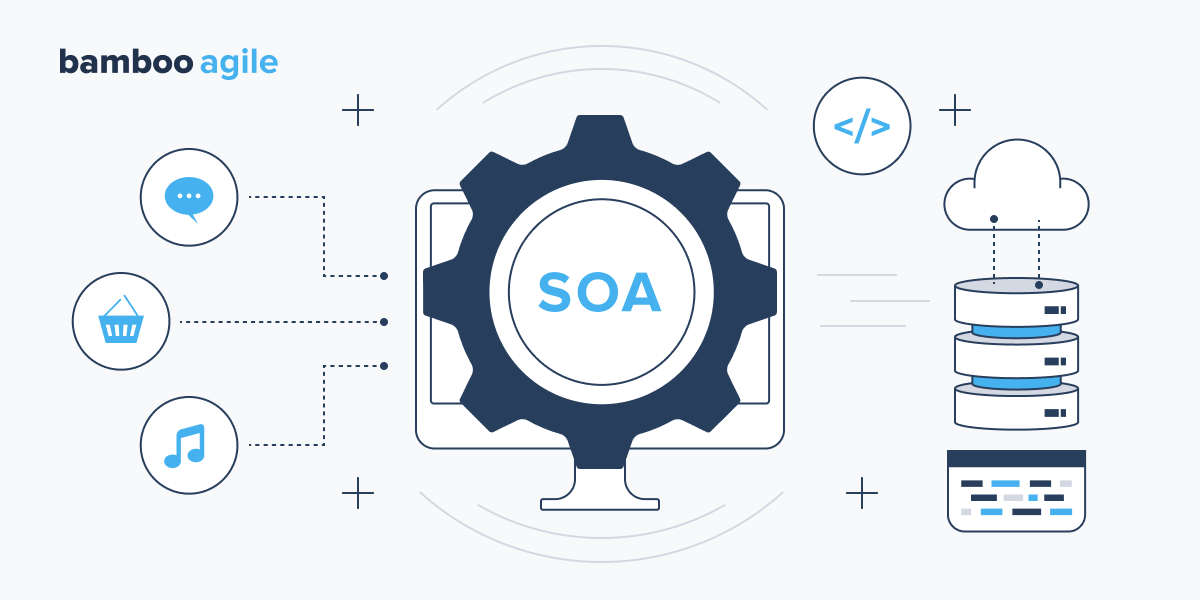
\includegraphics[width=0.8\textwidth]{imagenes/soa.png}
  \caption{Arquitectura orientada a servicios aplicada al sistema}
  \label{fig:ejemplo}
  \vspace{0.3cm}
  \small \textit{Fuente: Adaptado de Smith (2022) y \cite{doe2023}}
\end{figure}

\section{Justificación}

La necesidad de herramientas educativas accesibles y dinámicas ha crecido con el auge del aprendizaje remoto y personalizado. Integrar funcionalidades como generación automática de contenido y síntesis de voz permite a los usuarios con diferentes capacidades acceder a experiencias más inclusivas. Este proyecto responde a esa demanda desarrollando una solución moderna, basada en tecnologías web y servicios de IA.

\section{Objetivos del estudio}

Este informe tiene como objetivo principal documentar la implementación de un sistema web que combina una arquitectura desacoplada con servicios inteligentes. En el siguiente capítulo se detallan los objetivos específicos de este trabajo.
